\documentclass[10pt]{beamer}

\usetheme{metropolis}
\usepackage{appendixnumberbeamer}

\usepackage{booktabs}
\usepackage[scale=2]{ccicons}

\usepackage{pgfplots}
\usepgfplotslibrary{dateplot}

\usepackage{multimedia}

\usepackage{xspace}
\newcommand{\themename}{\textbf{\textsc{metropolis}}\xspace}

\graphicspath{ {./images/} } 

\title{DLS Lab annual seminar}
\subtitle{}
\date{March 16, 2017}
\author{Octavio Villarreal}
\institute{Istituto Italiano di Tecnologia}
\titlegraphic{\hfill
\includegraphics[height=0.5cm]{ADVRLogo.png}}

\begin{document}

\maketitle

\begin{frame}{Table of contents}
  \setbeamertemplate{section in toc}[sections numbered]
  \tableofcontents[hideallsubsections]
\end{frame}

\section{Introduction}
\begin{frame}{About me}
	\begin{columns}
		\begin{column}{0.6\textwidth}
		Octavio A. Villarreal Maga\~na
		\\
			\begin{itemize}\setlength\itemsep{2.5em}
				\item MSc. Mechanical Engineering, track Control Engineering (TUDelft, The Netherlands)
				\begin{itemize}\setlength\itemsep{1em}
					\item [--] Control Methods for Robotics
					\item [--] Robust Control
				\end{itemize}
				\item BSc. Mechatronic Engineering (UNAM, Mexico)
				\begin{itemize}\setlength\itemsep{1em}
					\item [--] Systems and Control
					\item [--] Robotics
				\end{itemize}
			\end{itemize}
		\end{column}
		\begin{column}{0.4\textwidth}
			\begin{figure}[ht]
				\vspace{-59.3pt}
				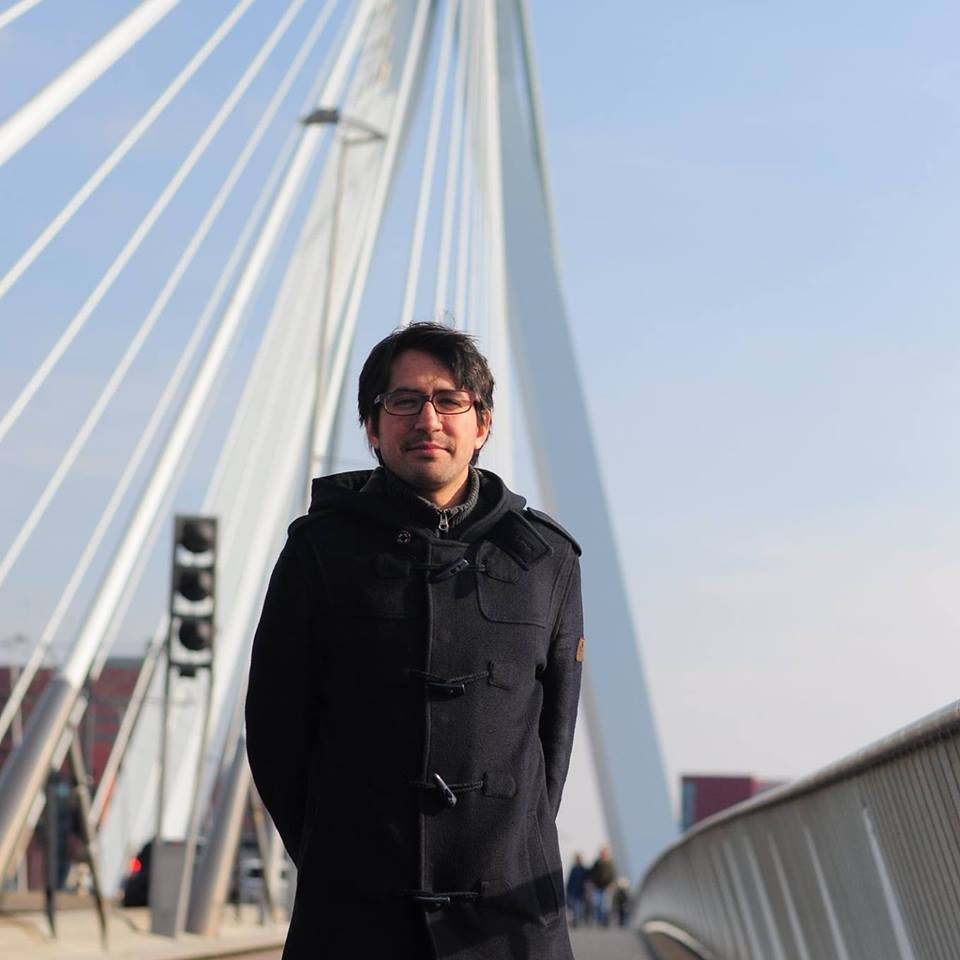
\includegraphics[width=1.5\textwidth]{images/yo.jpg}
			\end{figure}			
		\end{column}
	\end{columns}
\end{frame}
\section{Master thesis: "Dynamic control of 3D directional drilling systems using state estimation"}

\begin{frame}{Dynamic control of 3D directional drilling systems}
	\begin{itemize}\setlength\itemsep{2.5em}
		\item Challenging dynamic system
		\item Collaboration between researchers of TU Delft, TU Eindhoven and the University of Minnesota
		\item Little research on this field
	\end{itemize}
\end{frame}

\begin{frame}{Applications of directional drilling}	
	\begin{columns}
	\hspace{0.9cm}\begin{column}{0.4\textwidth}
	\begin{figure}[t]
		\centering
		\begin{minipage}[t]{1\textwidth}
			\centering
			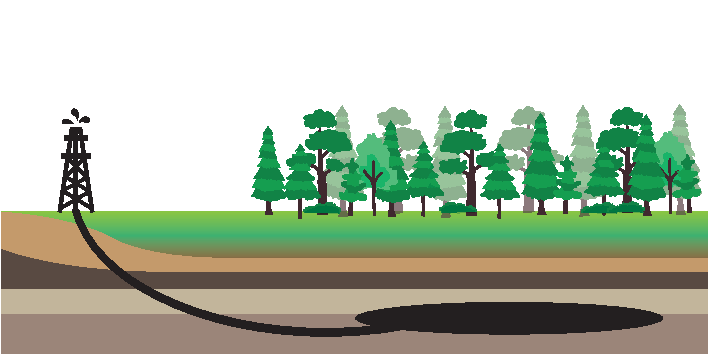
\includegraphics[width=1\linewidth]{images/appdd1.pdf}\\
		\end{minipage}%\\
		\\\begin{minipage}[t]{1\textwidth}
			\centering
			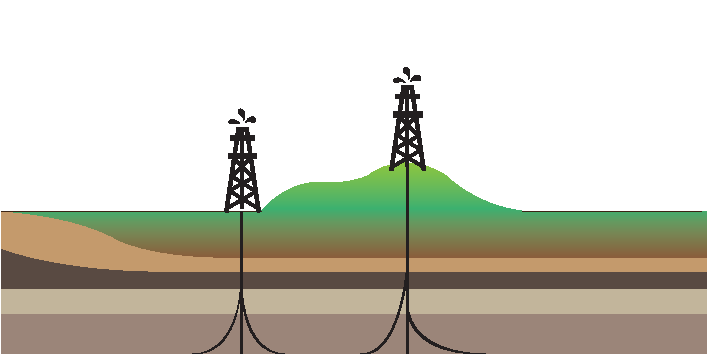
\includegraphics[width=1\linewidth]{images/appdd2.pdf}\\
		\end{minipage}
		\begin{minipage}[t]{1\textwidth}
			\centering
			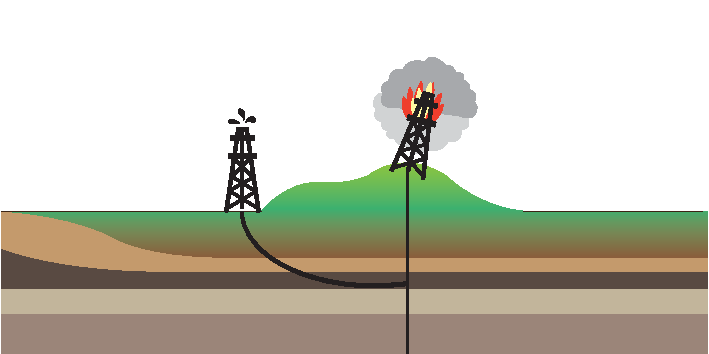
\includegraphics[width=1\linewidth]{images/appdd3.pdf}\\
		\end{minipage}
	\end{figure}
	\end{column}
	\begin{column}{0.6\textwidth}\setlength{\leftmargini}{20pt}
		\begin{itemize}\setlength\itemsep{2.5em}
			\item Extract oil, mineral and thermal energy resources
			\item Reach targets that need complex geometries such as:
				\begin{itemize}\setlength\itemsep{1em}
					\item Under a city or an ecosystem
					\item Far from the drill rig
					\item Relief for hazardous situations
				\end{itemize}
		\end{itemize}
	\end{column}
	\end{columns}
\end{frame}

\begin{frame}\frametitle{General description of the system}
	\begin{columns}
	\hspace{1cm}	\begin{column}{0.6\textwidth}
		\begin{figure}[ht]\centering
				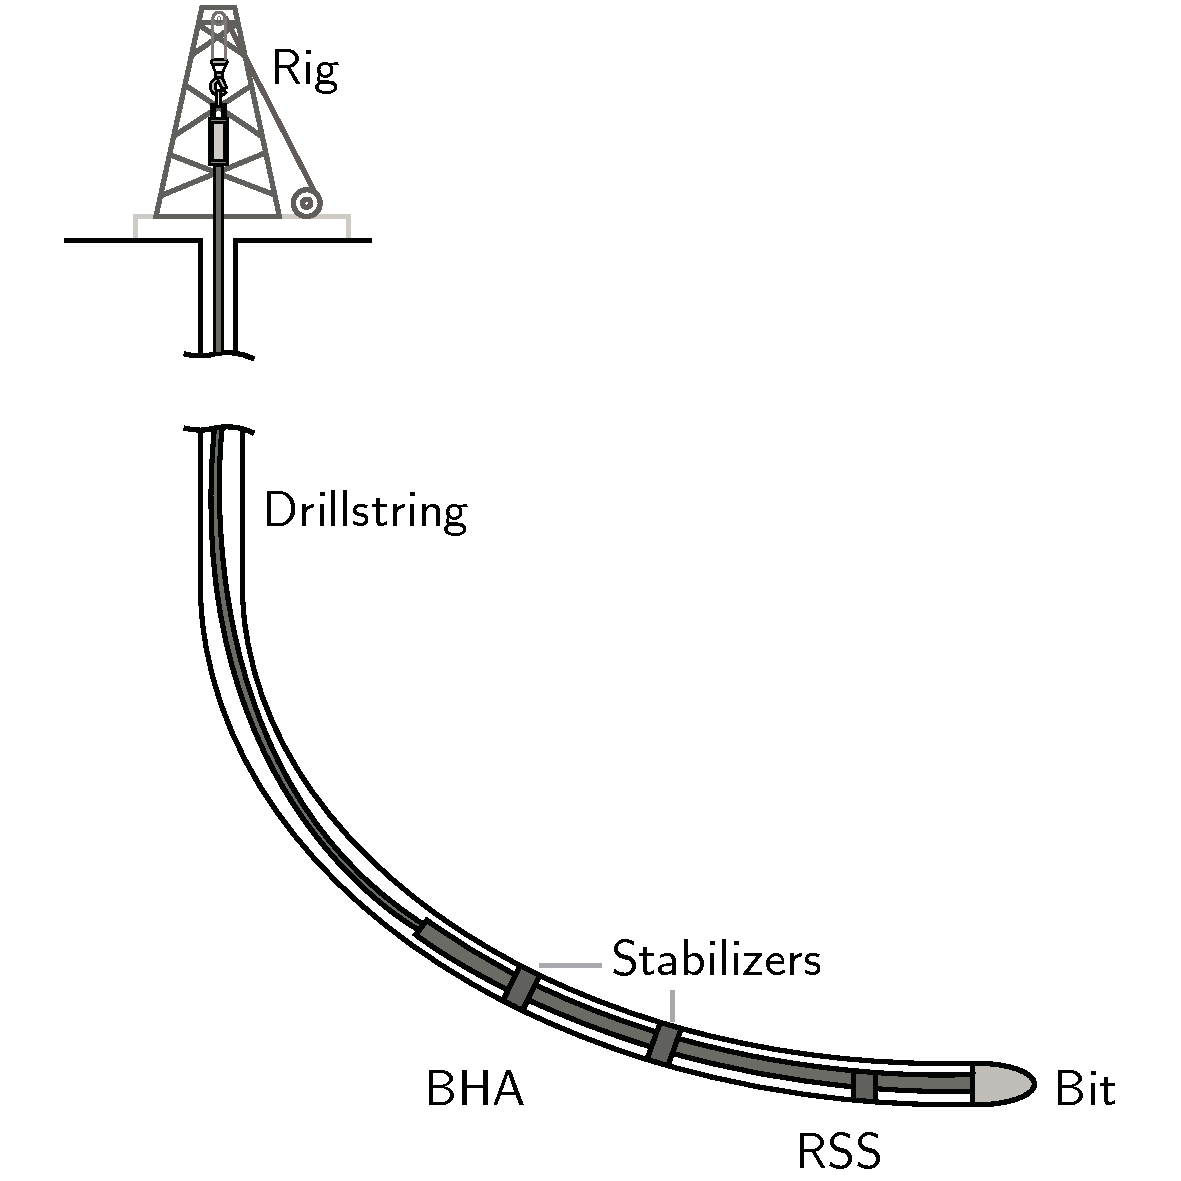
\includegraphics[width=1\textwidth]{images/drillingsystem.pdf}
			\end{figure}
			BHA: Bottom hole assembly
		\end{column}
		\begin{column}{0.4\textwidth}
			\centering
			Rotary Steerable System (RSS)
			\vspace{-10pt}	
			\begin{figure}[ht]
				\begin{minipage}[t]{1\textwidth}
				\hspace{0cm}	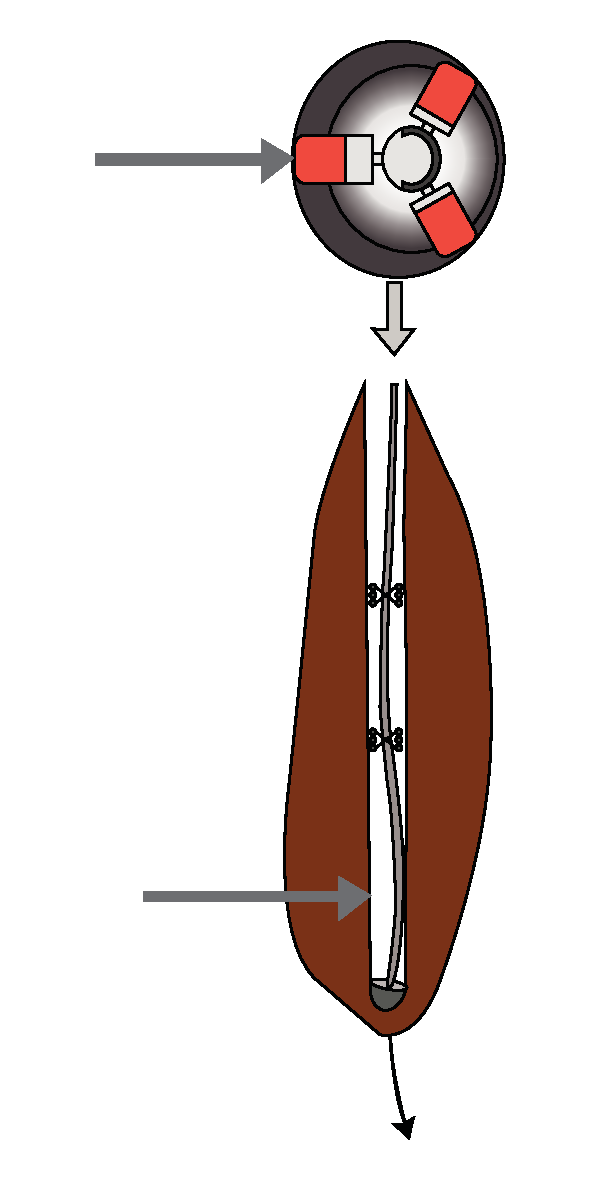
\includegraphics[width=0.65\textwidth]{images/RSS.pdf}
				\end{minipage}
			\end{figure}			
		\end{column}
	\end{columns}
\end{frame}

\begin{frame}{Context and challenges}
		\begin{columns}[T]
		\hspace{1cm}	\begin{column}{0.5\textwidth}\setlength{\leftmargini}{0pt}
				\vspace{1cm}
				\begin{figure}[ht]\centering
					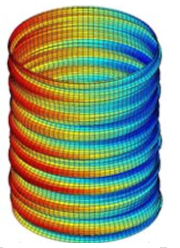
\includegraphics[width=0.5\textwidth]{images/Spiraling.png}
				\end{figure}
			\centering	[Sugiura 2009]
			\end{column}
			\begin{column}{0.6\textwidth}\setlength{\leftmargini}{0pt}
				\begin{itemize}
					\setlength\itemsep{3em}
					\item State-of-practice: Constant RSS force
					\item Negative effects: kinking, rippling and spiraling
					\item Consequences of negative effects: reduced penetration rate and accuracy
				\end{itemize}			
			\end{column}
		\end{columns}
\end{frame}

\begin{frame}{Research goals}
	\begin{block}{Main goal}\Large Develop a control strategy for a 3D directional drilling system, that allows to drill boreholes with complex geometries.
	\end{block}
\end{frame}

\begin{frame}{Previous works}
	\begin{itemize}\setlength\itemsep{1em}
		\item Model of 3D directional drilling systems [Perneder 2013]
		\item Model-based decoupled control of a 3D directional drilling system [Monsieurs 2015]
		\begin{itemize}\setlength\itemsep{1em}
			\item State-feedback controller
			\item Relies on availability of measurements of the states (not possible in practice)
		\end{itemize}
	\item []\begin{block}{Subgoals}	
	\begin{itemize}\setlength\itemsep{1em}
		\item Control strategy that relies only on local measurements
		\item Robustness against parametric uncertainty
	\end{itemize}
	\end{block}
	\end{itemize}
\end{frame}

\begin{frame}{Model charateristics}
\begin{columns}
\begin{column}{0.5\textwidth}
	\begin{itemize}\setlength\itemsep{1em}
	\item Function of (dimensionless) borehole length $\xi$
	\item Model form: nonlinear coupled delay differential equations (delays: BHA should fit in already drilled borehole)
	\item States: borehole inclination ($\Theta$) and azimuth ($\Phi$) at the bit
	\item No access to measurements of the states (output equations of sensors)
	\end{itemize}
\end{column}
	\begin{column}{0.4\textwidth}
	\begin{figure}[ht]\centering
		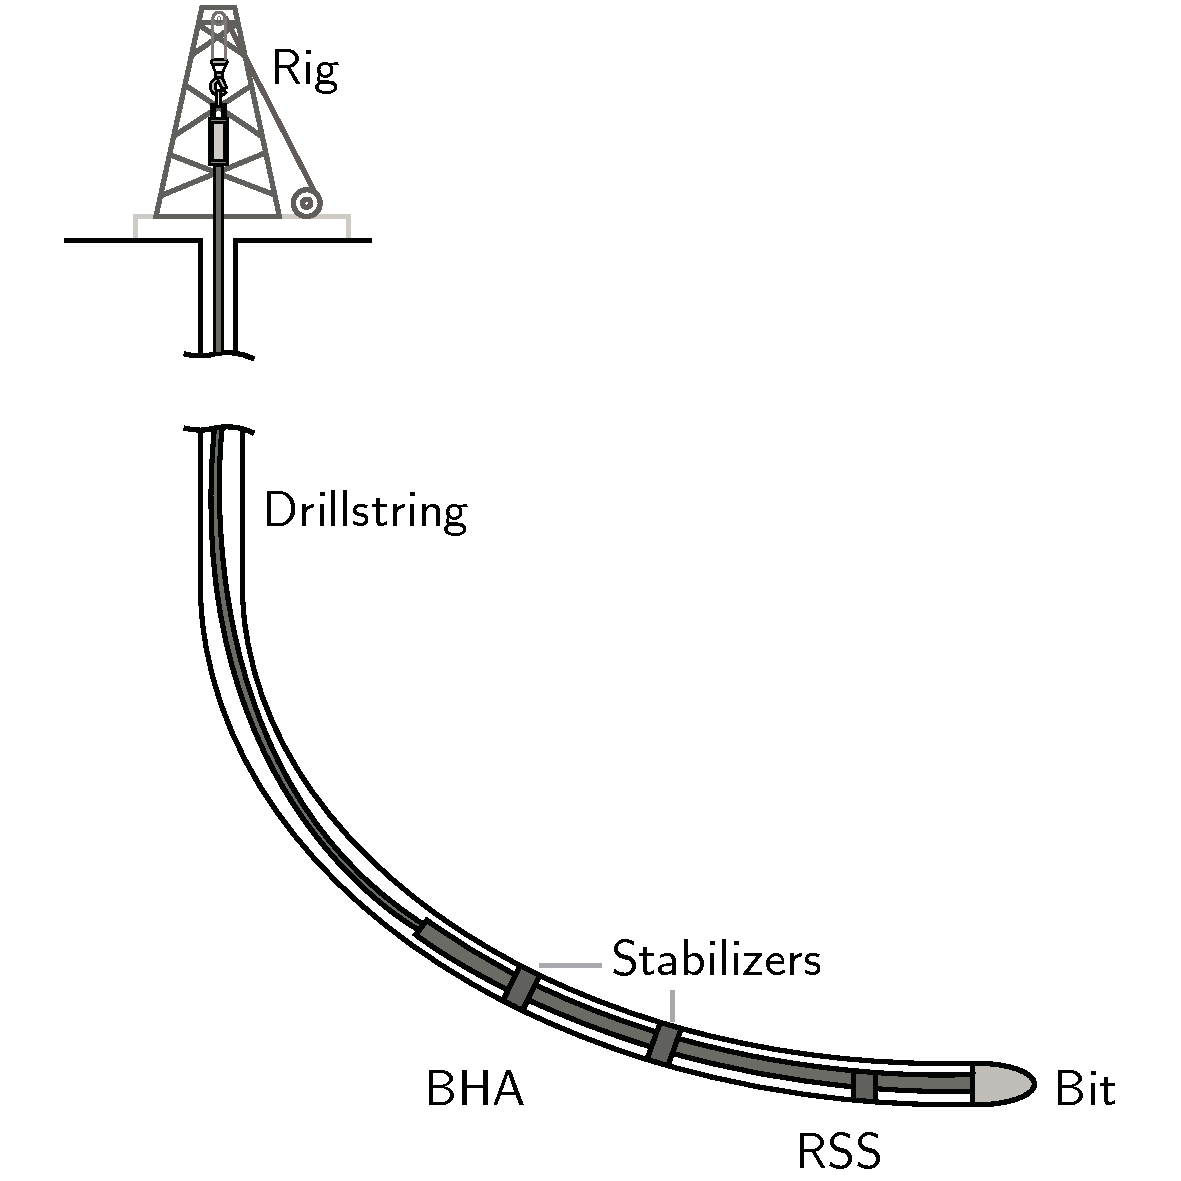
\includegraphics[width=1.25\textwidth]{images/drillingsystem.pdf}
	\end{figure}
	\end{column}
\end{columns}
\end{frame}

\begin{frame}{Available measurements}
	\begin{figure}[ht]\centering
				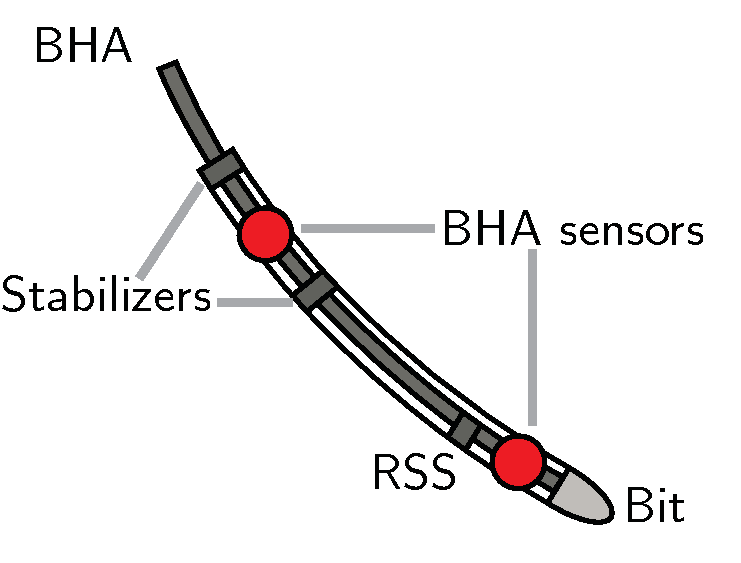
\includegraphics[width=0.8\textwidth]{images/Sensors.pdf}
	\end{figure}
\end{frame}


\begin{frame}{Control objectives}
	\begin{itemize}\setlength\itemsep{1.5em}
		\item Track a desired reference trajectory corresponding to a complex borehole geometry
		\item The response of the system should have favorable transient behavior (avoid kinking, rippling and spiraling)
	\end{itemize}
\end{frame}



\begin{frame}{Plant definition}\setlength{\leftmargini}{0pt}
\begin{itemize} 
				\item <1|only@1> [] \begin{figure}[ht]\centering
				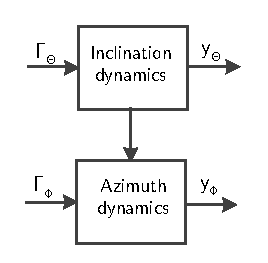
\includegraphics[width=0.7\textwidth]{images/Plant.pdf}
			\end{figure}
			\item <2|only@2> [] \begin{figure}[ht]\centering
				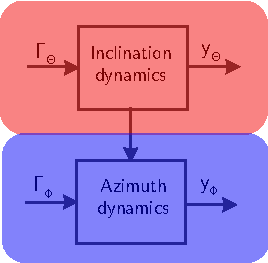
\includegraphics[width=0.7\textwidth]{images/Plant2.pdf}
			\end{figure}
\end{itemize}
\end{frame}

\begin{frame}{Output-feedback strategy}
	\begin{columns}
		\hspace{1cm}\begin{column}{0.5\textwidth}
			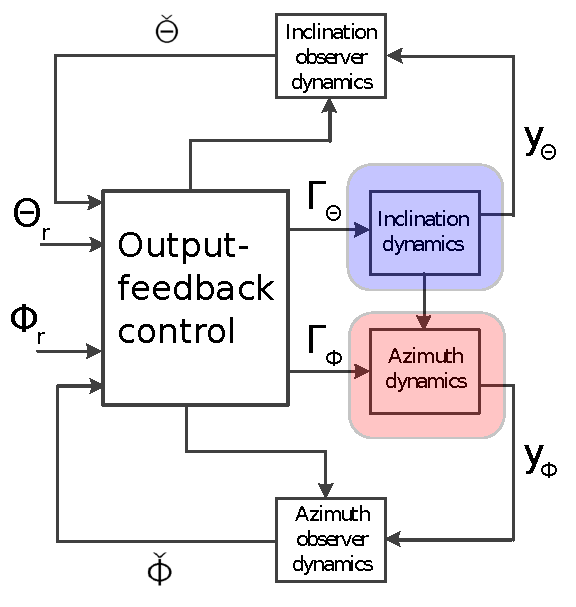
\includegraphics[width=1.1\textwidth]{images/ControlStrategyRobust.pdf}
			
			\footnotesize \begin{equation*}
						e_i := i_{r} - i \qquad \delta_i := i - \check{i}_i \quad \text{ for } i=\Theta,\Phi
			\end{equation*}
		\end{column}
		\begin{column}{0.5\textwidth}
			\begin{itemize}\setlength\itemsep{2.5em}
				\item Focus of the research: Include observer in the control structure
				\item Challenges
					\begin{itemize}
						\item  Nonlinear coupling between states while $\Theta \ne \check{\Theta}$
						\item  Controller and observer gain design
					\end{itemize}
			\end{itemize}
		\end{column}
	\end{columns}
\end{frame}

\begin{frame}{Controller synthesis}
\begin{itemize}\setlength\itemsep{0.9em}
	\item Define isolated systems $e_\Theta$, $\delta_\Theta$, $e_\Phi$ and $\delta_\Phi$
	\item Synthesize $K_\Theta$, $L_\Theta$, $K_\Phi$ and $L_\Phi$ for each isolated system separately
	\item Favorable transient performance
\end{itemize}
	\begin{figure}[ht]\centering
		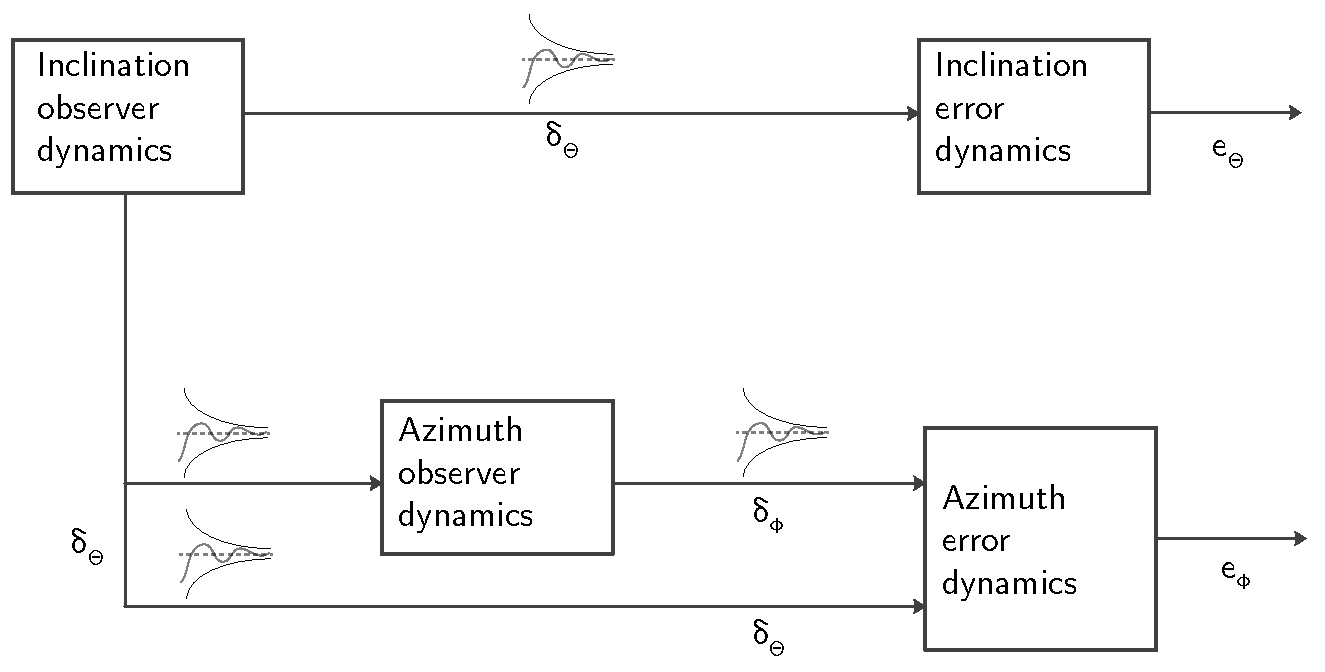
\includegraphics[width=0.85\textwidth]{images/ISS.pdf}
	\end{figure}
\end{frame}

\begin{frame}{Controller synthesis}
\begin{itemize}
	\item Infinite number of poles in delay systems (no pole-placement)
	\item Spectral approach [Michiels and Niculescu 2007]
	\item Optimize location of right-most pole over $K_i$ (state-feedback gain) and $L_i$ (observer-feedback gain)
\end{itemize}

\hspace{2.0cm} 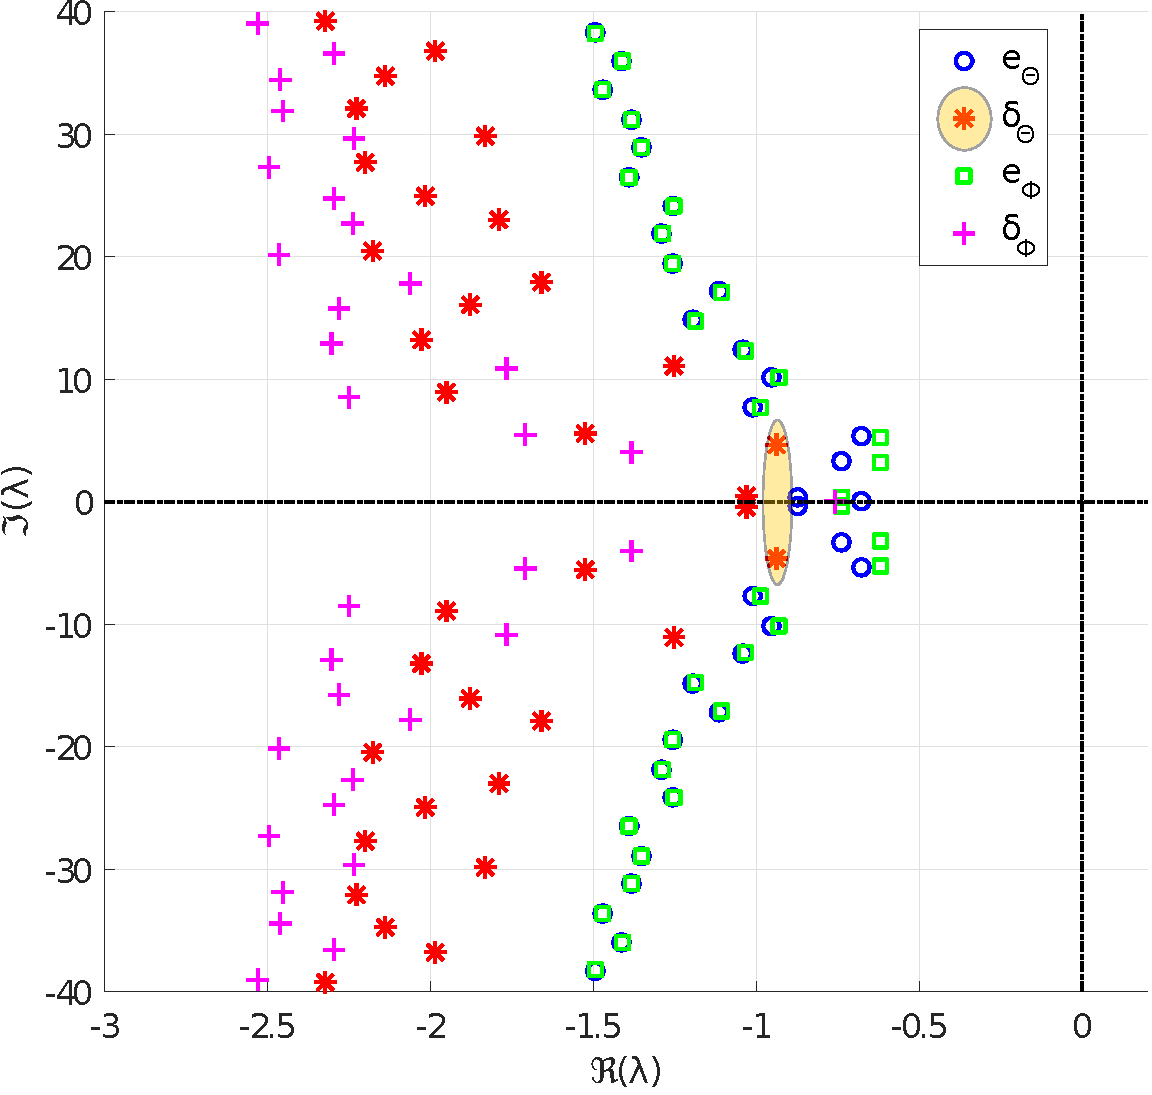
\includegraphics[width=0.6\textwidth]{images/ClosedLoopPolesNeutral.pdf}
\end{frame}

\begin{frame}{Simulation results}
\begin{figure}[t]
	\centering
	\begin{minipage}[b]{0.5\textwidth}
		\centering
		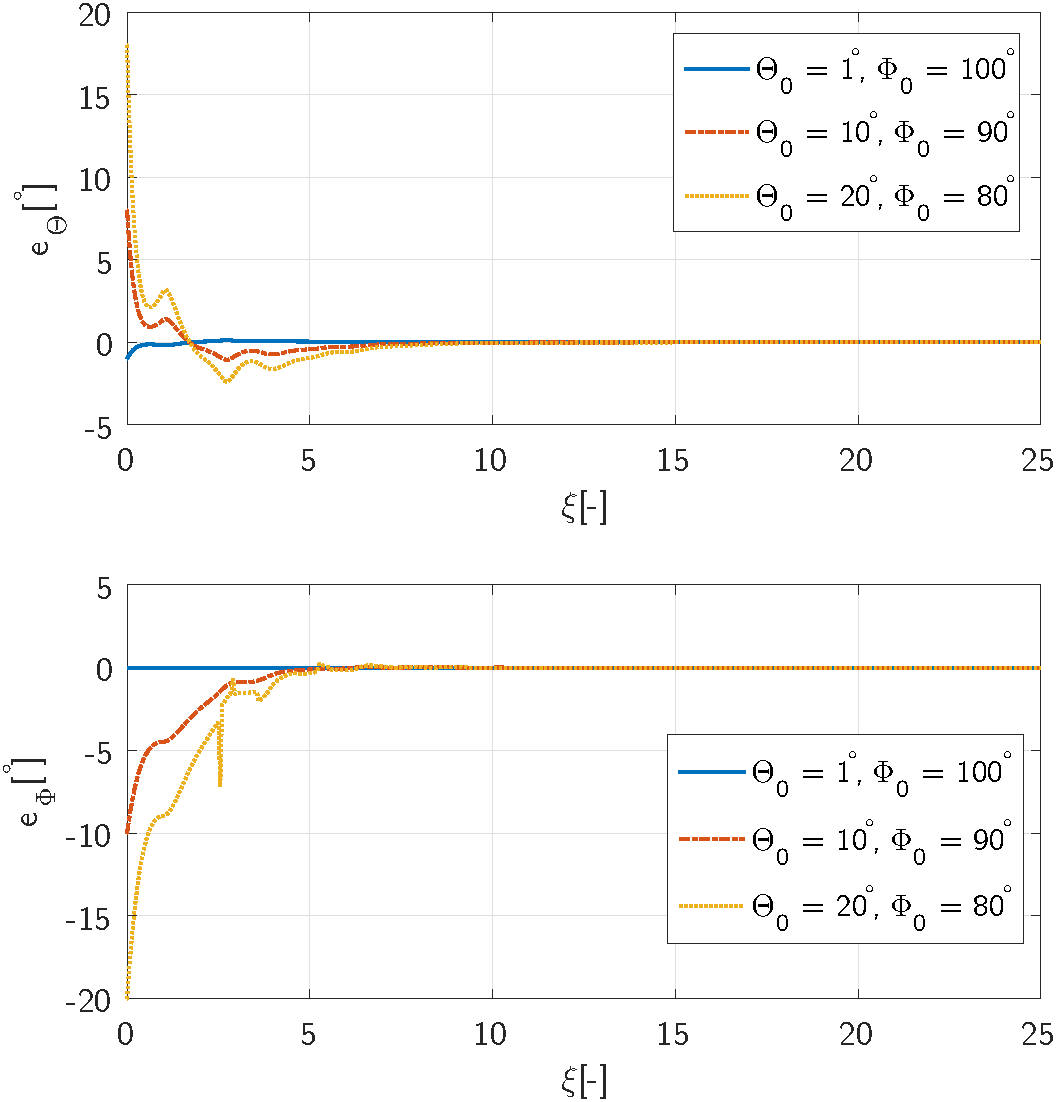
\includegraphics[height=1.1\textwidth]{ErrorsNeutral.pdf}
		\label{fig:ReferenceTrajectoryThetaPhi} 
	\end{minipage}
	\begin{minipage}[b]{0.45\textwidth}
		\centering
		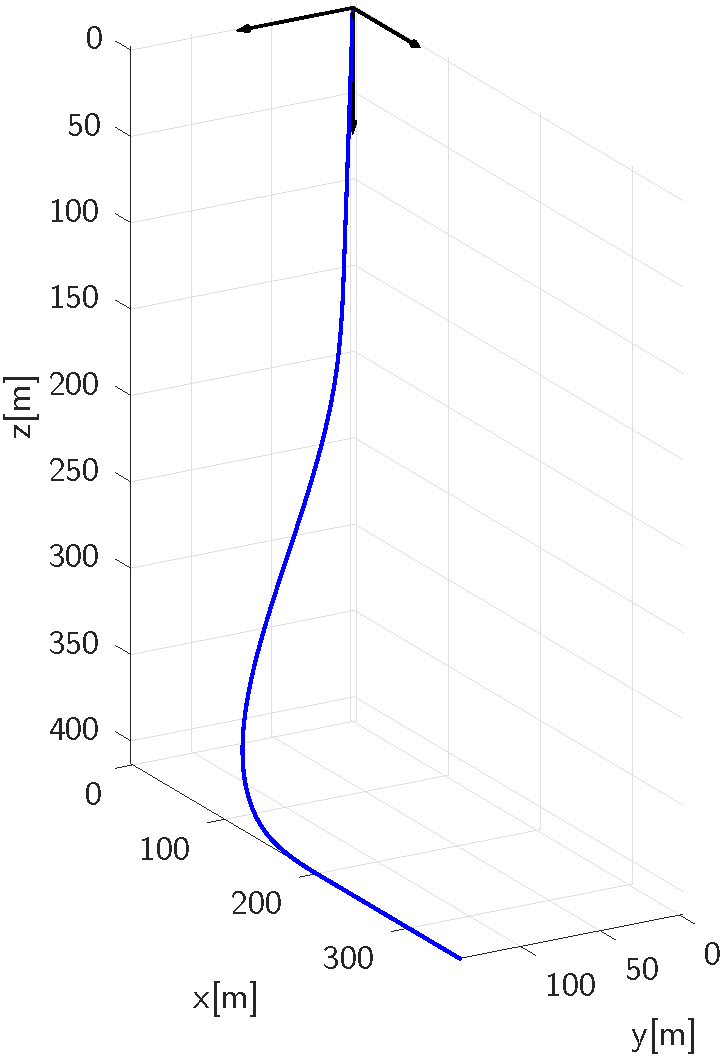
\includegraphics[height=2.3in]{ReferenceTrajectory.pdf}
		\label{fig:ReferenceTrajectoryV} 
	\end{minipage}
\end{figure}
\end{frame}

\section{Research proposal: "Locomotion control of HyQ using max-plus algebra linear systems"}

\begin{frame}{Motivation}
	\begin{itemize}\setlength\itemsep{3em}
		\item Provide versatility to the types of gaits that the robot can perform
		\item Have a unified and systematic way to generate motions of the legs according to the scenario
		\item Can be applied to other legged systems
	\end{itemize}
\end{frame}

\begin{frame}{General picture}	
	\begin{itemize}[notitemsep, topsep=0pt]
		\item <1|only@1> [] 
		\begin{figure}[ht]\centering
			\hspace{-25pt}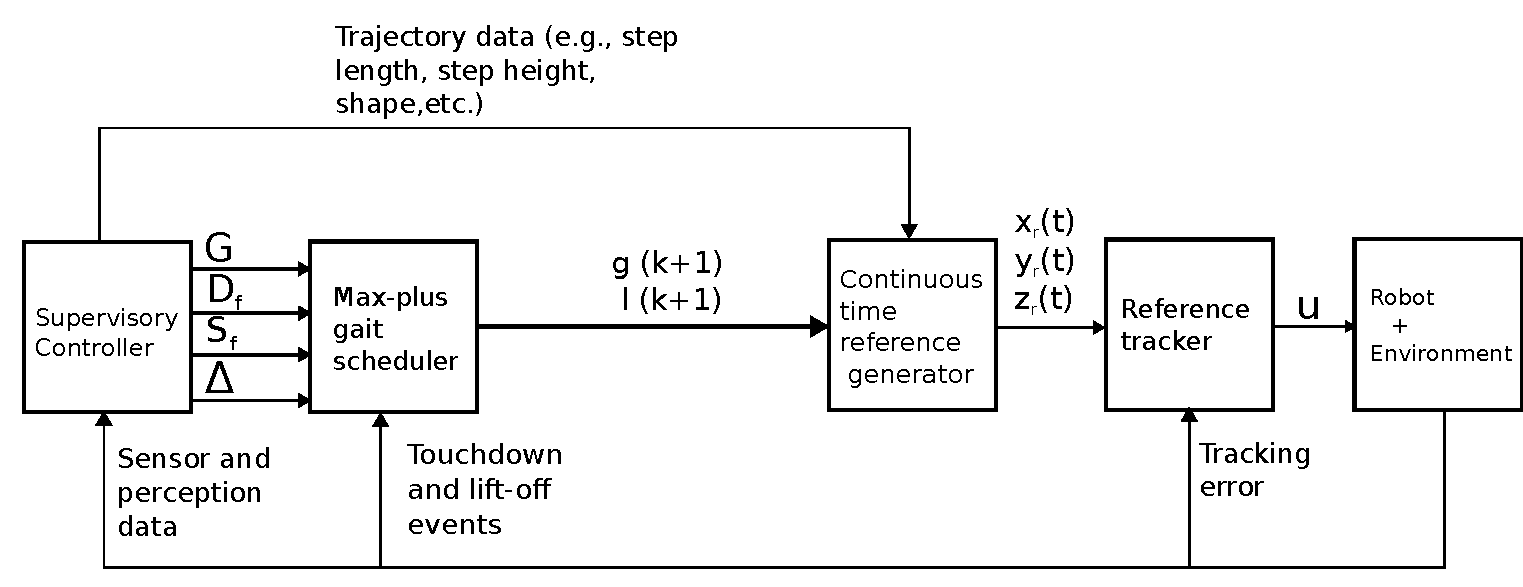
\includegraphics[width=1\textwidth]{images/ControlStrategy.pdf}
		\end{figure}
		\item <2|only@2> [] 
		\begin{figure}[ht]\centering
			\hspace{-25pt}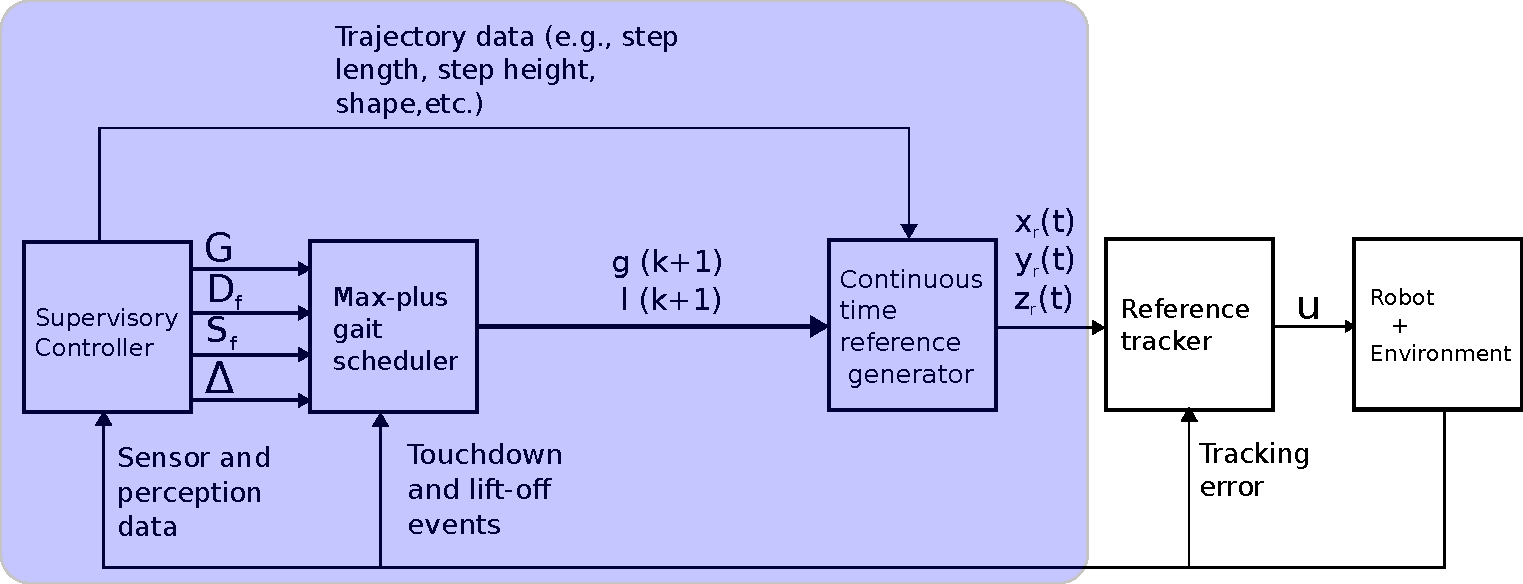
\includegraphics[width=1\textwidth]{images/ControlStrategy1.pdf}
		\end{figure}
	\end{itemize}
\end{frame}

\begin{frame}\frametitle{Supervisory controller}
	\begin{block}{Main goal}
		\Large Decide \textbf{geometrical} and \textbf{time} gait parameters, based on sensory data, to overcome the scenario that the robot is facing.
	\end{block}
	\begin{figure}[ht]\centering
		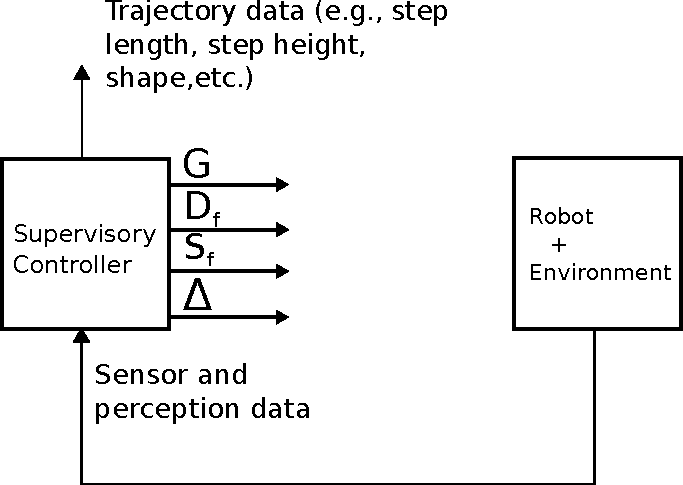
\includegraphics[width=0.5\textwidth]{images/Supervisory0.pdf}
	\end{figure}
\end{frame}



\begin{frame}{Geometrical parameters}
		\begin{columns}
		\hspace{1cm}
		\begin{column}{0.5\textwidth}
		
		\begin{itemize}
			\setlength\itemsep{3em}
			\item Not necessarily the same for all four legs
			\item Examples of trajectory parameters:
			\begin{itemize}
			\item Oscillator shape parameters [Barasuol et.al. 2013]
			\item Control points of a Bézier curve [Hyun et.al. 2014]
			\end{itemize}
			
		
		\end{itemize}	
		
		\end{column}
		\begin{column}{0.5\textwidth}
			\begin{figure}[ht]\centering
				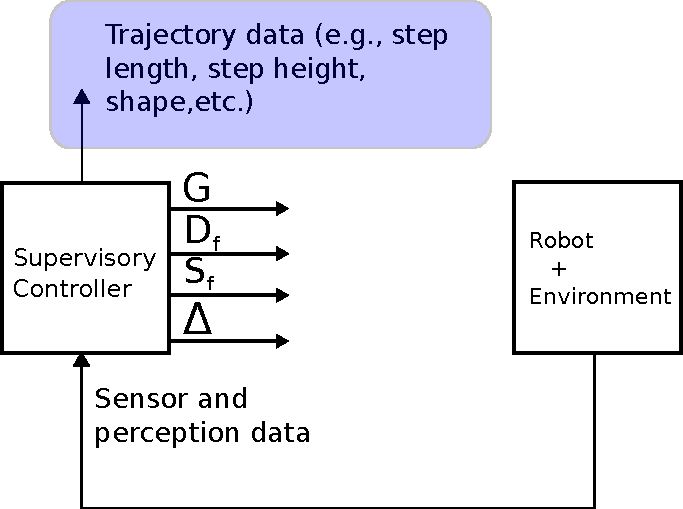
\includegraphics[width=0.75\textwidth]{images/Supervisory.pdf}
			\end{figure}
			\begin{figure}[ht]\centering
				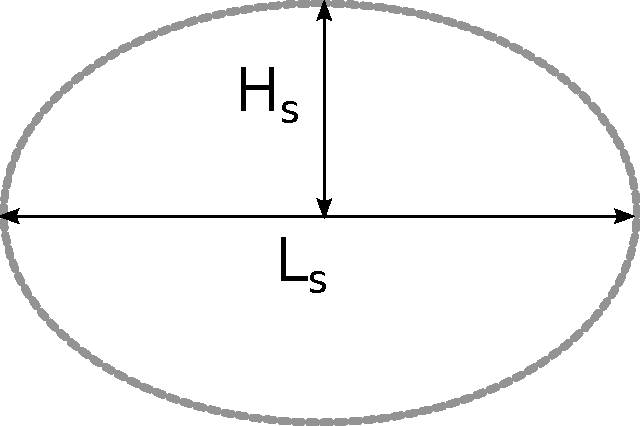
\includegraphics[width=0.75\textwidth]{images/PrimitiveShape.pdf}
			\end{figure}	
		\end{column}
		\end{columns}
	\end{frame}

\begin{frame}{Supervisory controller (continue)}
		\begin{columns}
		\hspace{1cm}
		\begin{column}{0.5\textwidth}
		Time parameters:
		\begin{itemize}
			\setlength\itemsep{3em}
			\item Duty factor $D_f$
			\item Step frequency $S_f$
			\item Gait parameterization $G$ (e.g., $G_{trot}=\{1,4\}\prec\{2,3\}$)
			\item Time difference vector $\Delta$
		\end{itemize}	
		
		\end{column}
		\begin{column}{0.5\textwidth}
			\begin{figure}[ht]\centering
				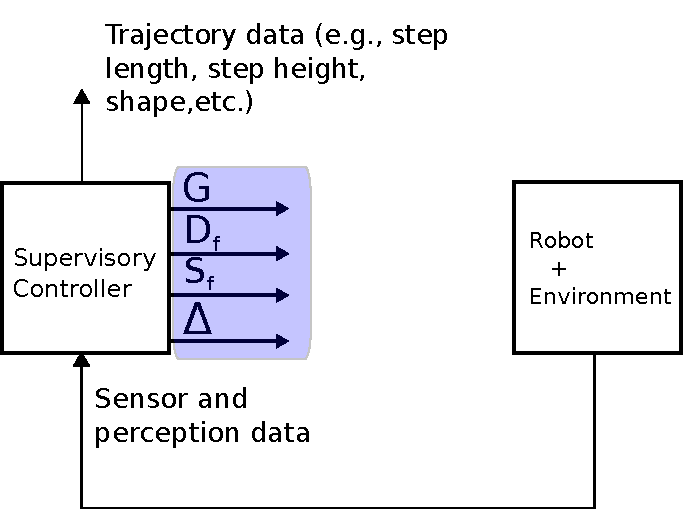
\includegraphics[width=0.6\textwidth]{images/Supervisoryb.pdf}
			\end{figure}
			\vspace{-0.25cm}\begin{figure}[ht]\centering
							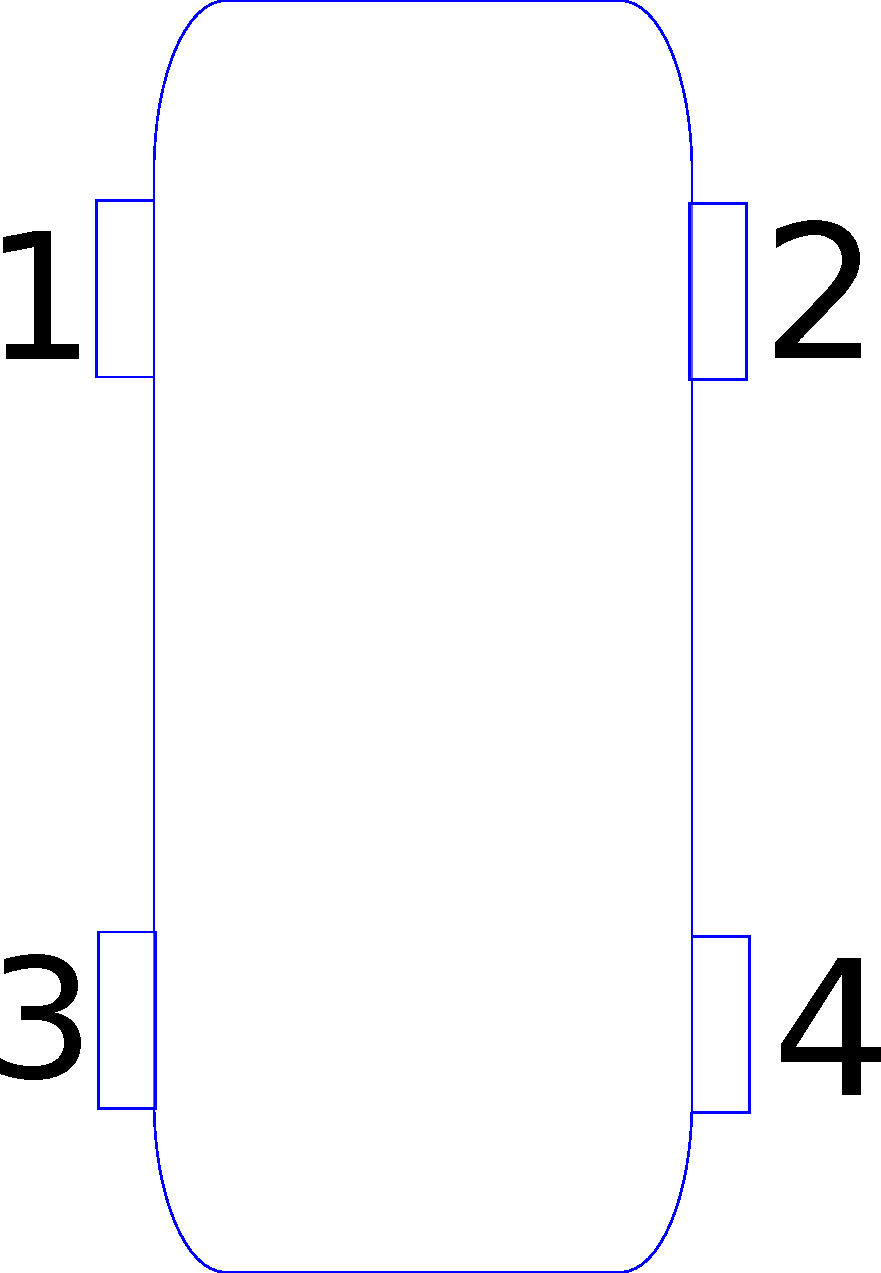
\includegraphics[width=0.22\textwidth]{images/Numbers.pdf}
			\end{figure}
			\begin{figure}[ht]\centering
				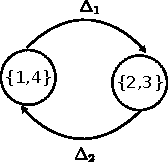
\includegraphics[width=0.45\textwidth]{images/TrotTime.pdf}
			\end{figure}
		\end{column}
		\end{columns}
\end{frame}

\begin{frame}{Max-plus gait scheduler}
	\begin{block}{Main goal}
		\Large Using the \textbf{time}-related gait parameters provided by the supervisory controller, generate the times that each leg has to touch or leave the ground.
	\end{block}
	\begin{figure}[ht]\centering
		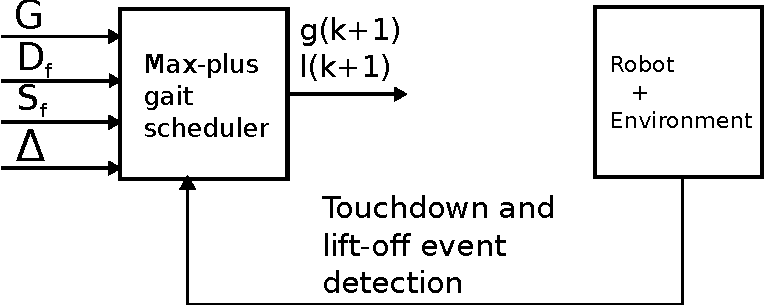
\includegraphics[width=0.8\textwidth]{images/MaxPlus.pdf}
	\end{figure}
\end{frame}

\begin{frame}{Max-plus gait scheduler (continue)}
\begin{columns}

\begin{column}{0.45\textwidth}

	\begin{figure}[ht]\centering
		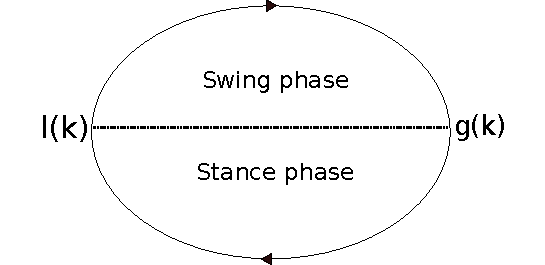
\includegraphics[width=1\textwidth]{images/Phases.pdf}
	\end{figure}
\end{column}
\begin{column}{0.55\textwidth}
$G_{trot}=\{1,4\}\prec\{2,3\}$ \\
$D_f = 0.58$ \\
$S_f = 0.42$ \\
$\Delta = [0.2,0.2]$ 

\begin{table}[]
\centering
\label{my-label}
\resizebox{\textwidth}{!}{\begin{tabular}{|l|l|l|l|l|l|l|l|l|}
\hline
$k$ & $g_1(k)$ & $g_2(k)$ & $g_3(k)$ & $g_4(k)$ & $l_1(k)$ & $l_2(k)$ & $l_3(k)$ & $l_4(k)$ \\ \hline
0   & 0        & 0        & 0        & 0        & 0        & 0        & 0        & 0        \\ \hline
1   & 2.4      & 3.6      & 3.6      & 2.4,     & 1.4      & 2.6      & 2.6      & 1.4      \\ \hline
2   & 4.8      & 6        & 6        & 4.8      & 3.8      & 5        & 5        & 3.8      \\ \hline
3   & 7.2      & 8.4      & 8.4      & 7.2      & 6.2      & 7.4      & 7.4      & 6.2      \\ \hline
4   & 9.6      & 10.8     & 10.8     & 9.6      & 8.6      & 9.8      & 9.8      & 8.6      \\ \hline
5   & 12       & 13.2     & 13.2     & 12       & 11       & 12.2     & 12.2     & 11       \\ \hline
\end{tabular}}
\end{table}
\end{column}
\end{columns}
\end{frame}

\begin{frame}{Max-plus gait scheduler (continue)}
\begin{itemize}
	\setlength\itemsep{2em}
	\item Systematic coordinated gait generation 
	\item Total cycle time analysis (max-plus linear systems theory)
	\item Coupling time analysis ("settling time")
	\item Not computationally expensive
\end{itemize}	
\end{frame}

\begin{frame}{Continuous reference generator}
	\begin{block}{Main goal}
		\Large Making use of the \textbf{touchdown} and \textbf{lift-off} times of the max-plus gait scheduler, provide a reference trajectory for each of the legs.
	\end{block}
	\begin{figure}[H]
		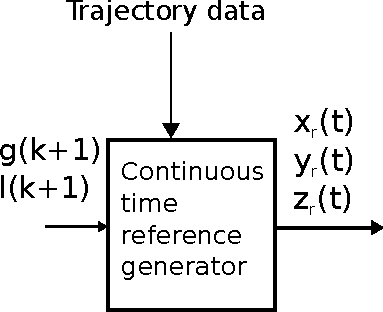
\includegraphics[width=0.5\textwidth]{AngularFrequency.pdf}
	\end{figure}
\end{frame}

\begin{frame}{Continuous reference generator}
Possible alternatives:
\begin{itemize}\setlength\itemsep{2em}
	\item Oscillator with angular frequency modulation according to max-plus scheduler
	\item Parameterized velocity profile using lift-off $l(k+1)$ and touchdown $g(k+1)$ as initial and final times respectively
\end{itemize}
\end{frame}

\begin{frame}{Simulations}
Change gait parameters every 20 seconds
\begin{figure}[H]\centering
	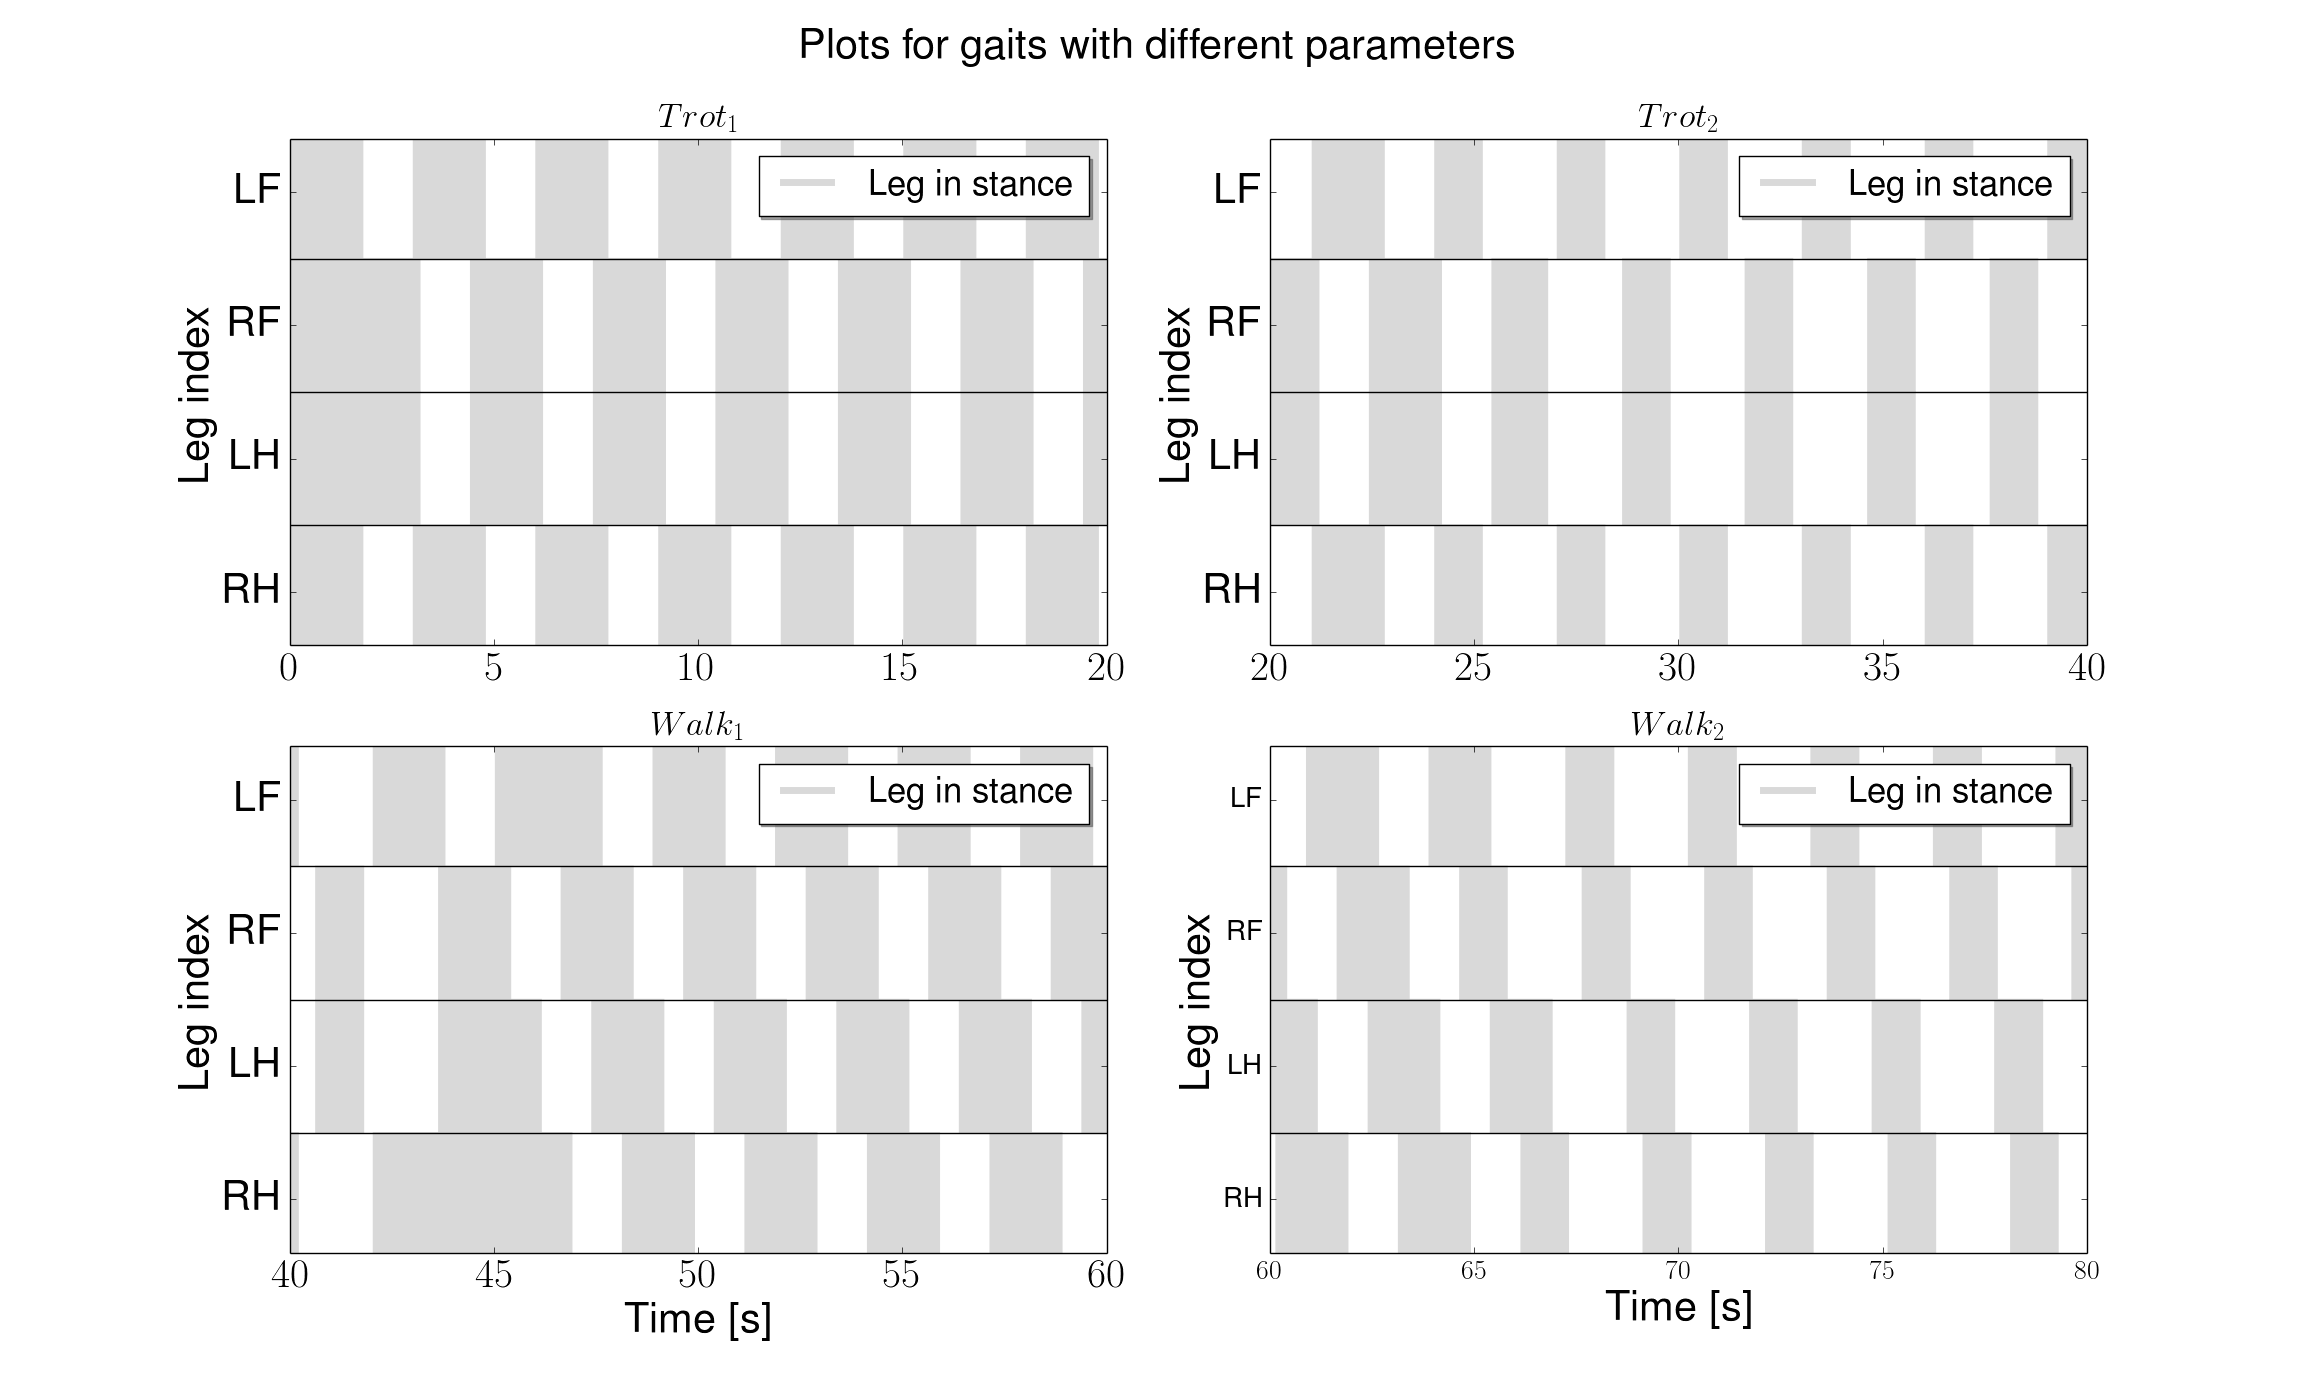
\includegraphics[width=1\textwidth]{SyncPlot.png}
\end{figure}
\end{frame}

\begin{frame}{Duty factor}
\vspace{-1cm}
	\begin{figure}[ht]\centering
		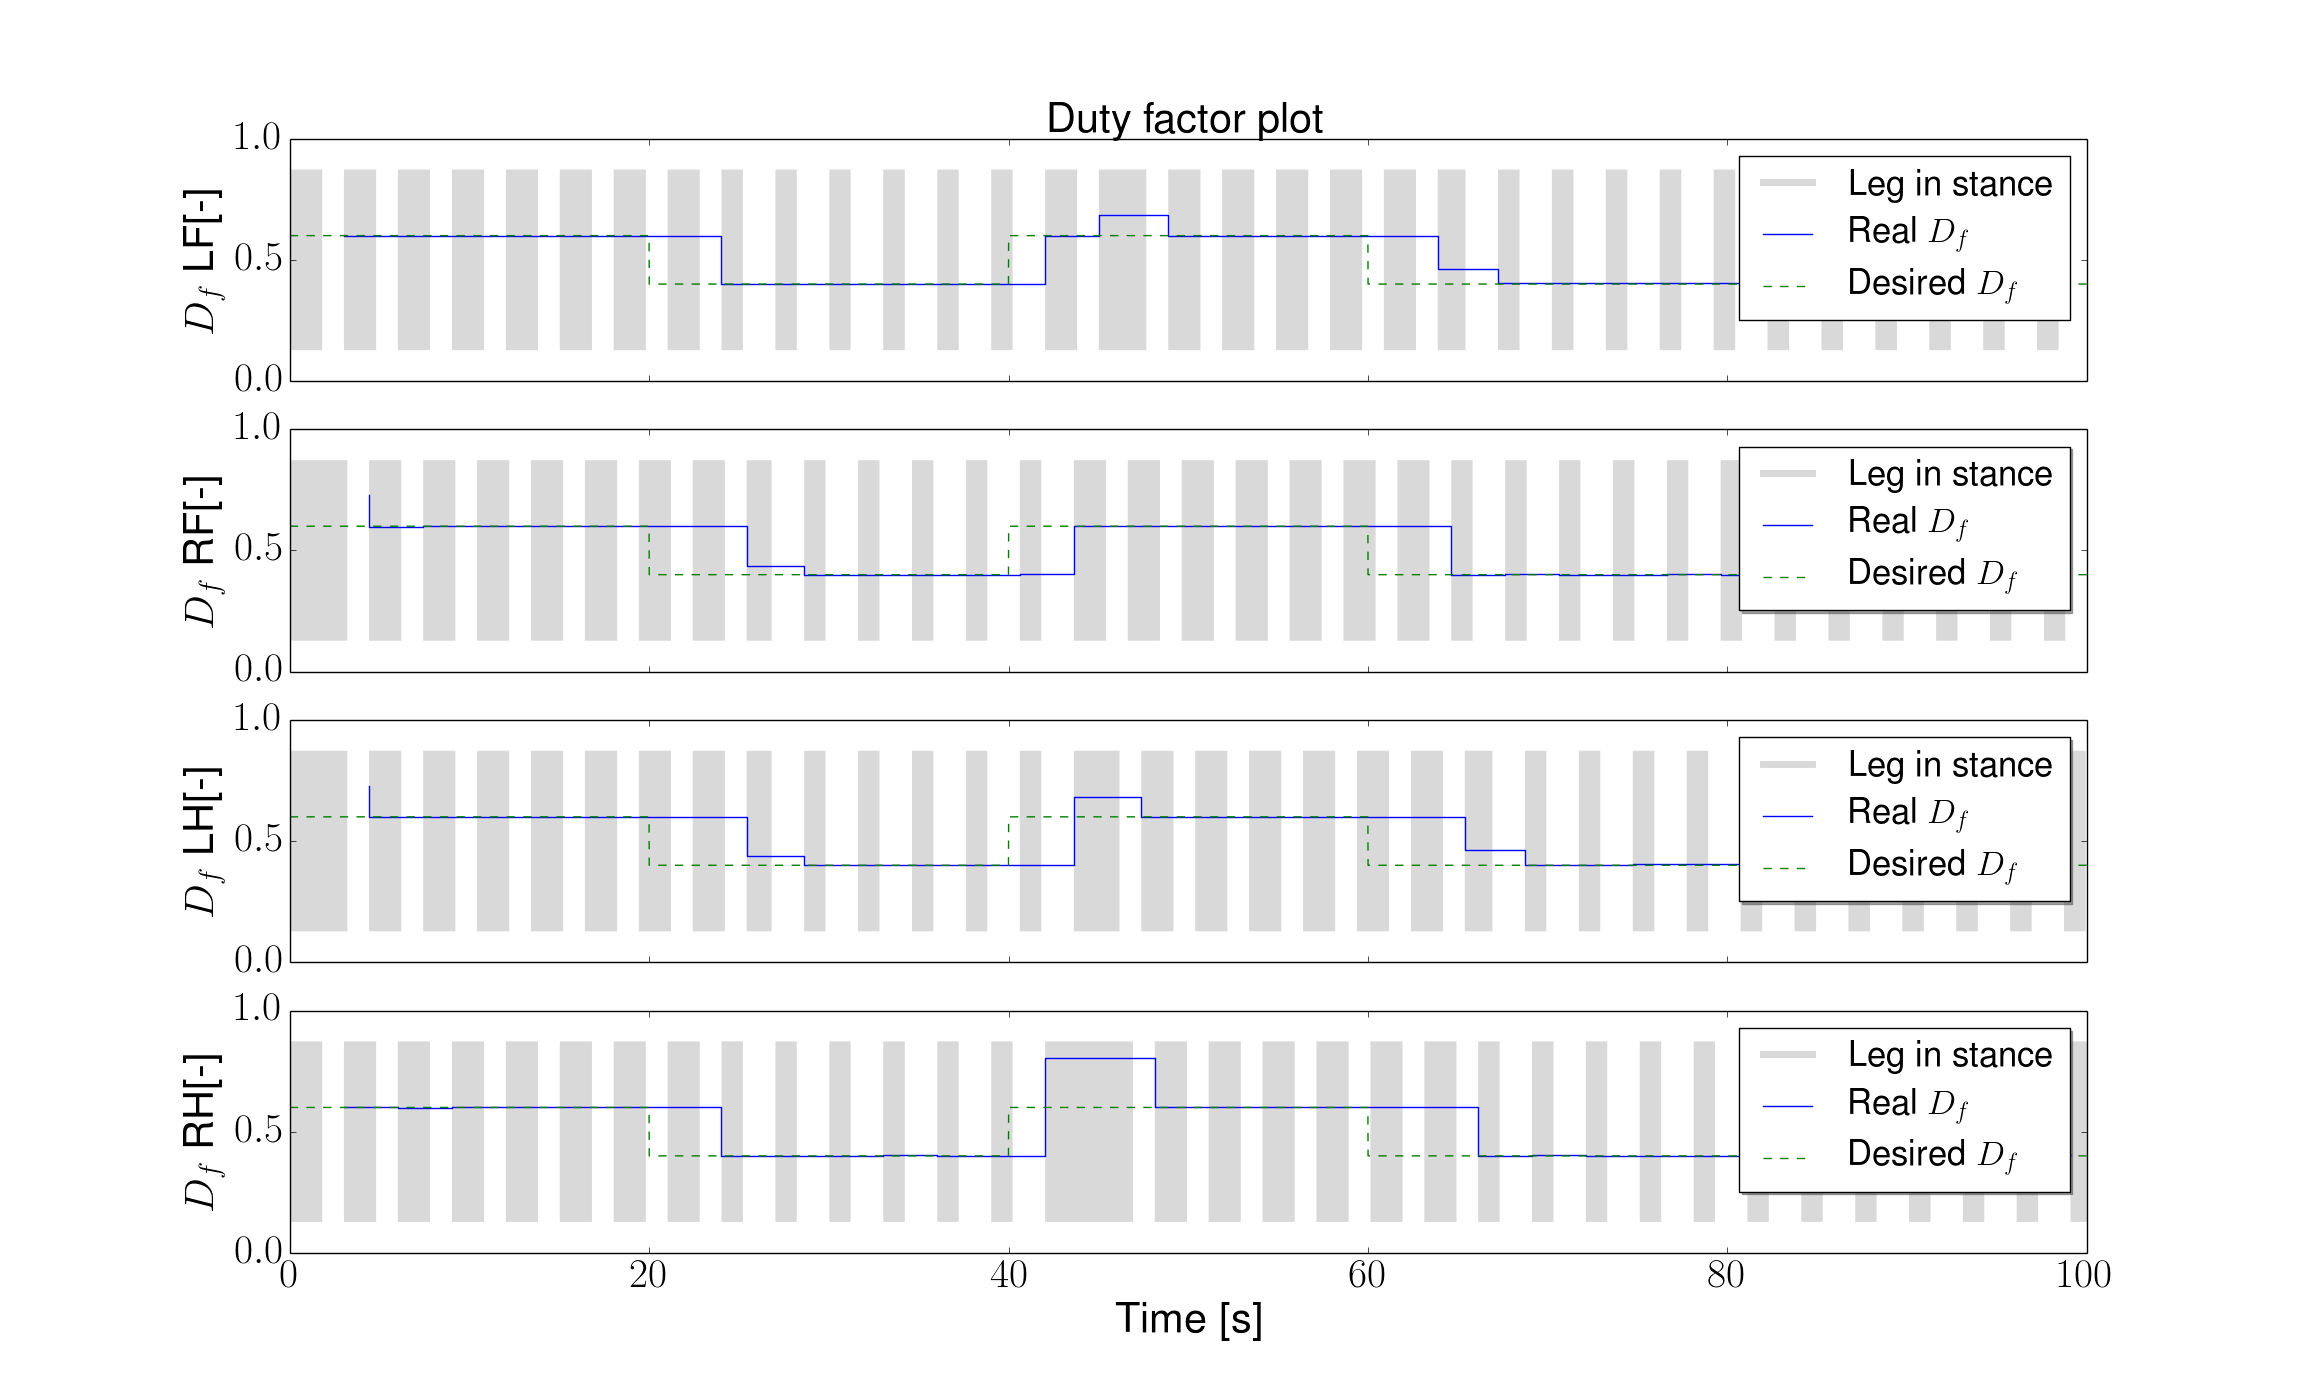
\includegraphics[width=1.1\textwidth]{images/DutyFactor.png}
	\end{figure}\vspace{-20pt}
\end{frame}

\begin{frame}{Animation}

\begin{center}
        \movie[width=\textwidth,showcontrols=true]
       {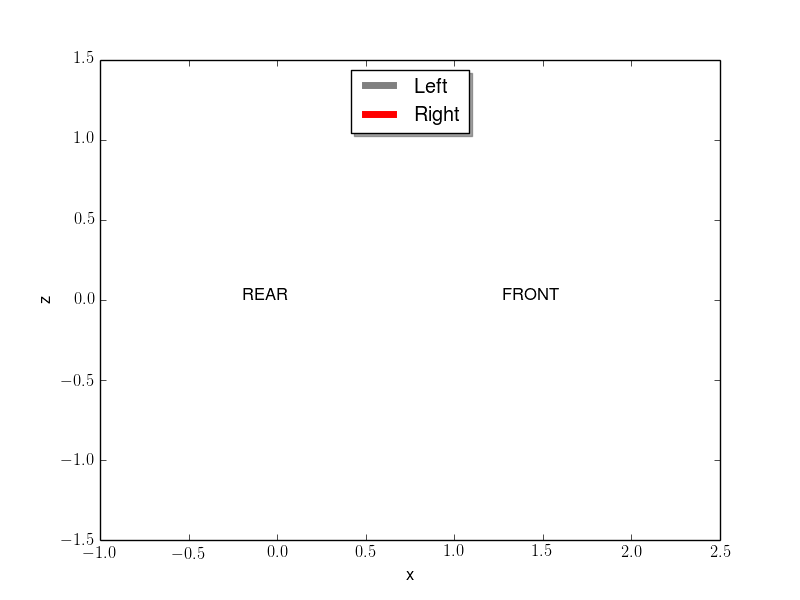
\includegraphics[width=\textwidth]{Legs.png}}{Legs.mp4} \\
\end{center}

\end{frame}


\begin{frame}
 \hspace{2cm} Thank you. Questions or comments?
\end{frame}


\end{document}
